To satisfy the computational needs of scientific algorithms, it is increasingly
necessary to parallelise their solution on modern multi-core CPUs, and GPUs. In
the past ten years since the first release of the CUDA language extension for
C/C++ the GPUs became widely used for high performance and scientific
computations. CUDA provides a low level abstraction commonly referred to as
Single Instruction Multiple Threads (SIMT), which gives us fine grained control
over GPU architectures. \\
A significant class of scientific applications operate on unstructured meshes,
which are represented as sets and explicit connections between them. These
applications are operating on large sets and usually execute similar
computations for every set element. For processing the elements, they can
access data on the set which they operate on, or, using indirections, data
defined on other sets. In the latter case multiple threads may try to modify
the same data, leading to race conditions. This algorithmic pattern is the
focus of our work: operations on sets that read and most importantly
\emph{increment} data indirectly on other sets. These operations are common in
numerical PDE solvers, such as Finite Volumes and Finite Elements. The adoption
of GPUs for these kind of computations could lead to considerable speedups due
to the highly parallel execution of the code. However, the straightforward
parallelisation of the scientific algorithms may not lead to optimal
performance on GPUs. The SIMT abstraction exposes a number of techniques that
can improve performance, one of which is the explicit management of the memory
system of the GPU.\\
The proper usage of the memory system for simulations is crucial to get good
performance. The latency of global memory accesses is a bottleneck for a lot of
kernels in modern scientific computations, thus we have to lower the impact of
the memory transactions. Since we can't fully hide the latency with
computations, we can either increase the number of memory transactions in
flight (to more efficiently utilise bandwidth), or decrease the number of
memory transactions with high latency. To achieve the latter goal we can use
shared memory for CUDA thread blocks as an explicitly managed cache, because it
has much lower latency than global memory. However, to get good performance we
have to ensure that we can use these memories efficiently from all threads in
the blocks.

Most codes do one of two things: they use a straightforward parallelisation
relying on either colouring or large temporary datasets to avoid two threads
that run simultaneously accessing the same data, but these end up with poor
data locality for most of the cases: one cannot have good reuse in reading
data, but no conflicts (and no reuse) in writing it. The only advantage of this
approach is that the parallelisation is simple, which means that it has lower
overhead at the beginning to plan the execution of the kernel. However, if we
spend more time for planning the execution strategy for the kernel, for example
by altering the order in which the elements are processed we can significantly
improve data locality. Better memory locality means that we can use cache lines
more efficiently (with one read transaction we can read multiple pieces of data
that we can use for the simulation) so that we end up with fewer memory
transactions in total, which means less time spent waiting for data.\\
Reordering and partitioning algorithms are already used for maximising data
reuse in CPUs and minimising communication in distributed memory systems. In
our work we use them to improve the data locality on GPUs, specifically within
CUDA thread blocks, to get better performance. We make the following
contributions:
\begin{enumerate}
  \item
    We adopt a caching mechanism on the GPU that loads indirectly accessed
    elements into shared memory. We use hierarchical colouring to avoid data
    races.
  \item
    We design a reordering algorithm based on partitioning that increases data
    reuse within a thread block, also increasing shared memory utilisation.
  \item
    We implement a library that parallelises applications on unstructured meshes
    and is capable of reordering the threads to increase efficiency.
  \item
    We analyse the performance of various parallelisations and data layout
    approaches on several representative applications and GPUs.
\end{enumerate}
The rest of the paper is structured as follows: the rest of Section
\ref{introduction} introduces the basic concepts of unstructured meshes and
also discusses some related works, Section \ref{parallelisation-on-gpu}
describes the used algorithms and the motivation behind them, Section
\ref{library-implementation} shows the structure of our library, then Section
\ref{measurements} shows the test-cases and the measurements we performed.
Finally, in Section \ref{conclusion}, we draw some conclusions from the
measurements.

\subsection{Background}\label{sec:background}
\subsubsection{Unstructured meshes}\label{unstructured-meshes}

\noindent Unstructured meshes can be abstractly viewed as a collection of sets 
(e.g. nodes, edges, cells, etc.), data defined on these sets (e.g. fluxes, 
coordinates, velocities), and explicit connectivity information between 
sets. The connectivity information, declared as mapping tables are required for 
determining the neighbors of a set element. If we represent sets as consecutive 
indices from zero to the size of the set, then the mapping between two 
sets is represented as an array which stores the index of set elements in the 
second set of the mapping (referred to as the to-set) for every set element of 
the first set (known as the from-set). For the majority of such applications, the number of to-set elements connected to each from-set element is fixed (e.g. all edges have two vertices). For example consider the mesh illustrated 
in Figure~\ref{fig:unstructured}. Figure~\ref{fig:mapping} details how part of 
the mappings from edges to cells are defined for this mesh. Given such a 
mapping, we can access the index of those elements which are connected to the 
current element of the from-set from other sets (the to-sets of the mappings). 

The computations on the mesh are declared as a loop over the elements of a set, 
executing some block of computation on each set element (i.e. an elemental kernel), 
while accessing data directly on the iteration set or indirectly through a 
mapping.  If a loop over a set only write to data defined on that set during the 
elemental kernel, then each iteration of the loop could run in parallel. 
However, for kernels which indirectly increment data, there may be multiple 
from-set iterations that update the same to-set element. Such indirect-loops are 
common in finite volume and finite element applications over 
unstructured-meshes: e.g. when updating state variables in cells using fluxes 
across faces, or when doing matrix assembly. The parallelization of indirect 
loops are non-trivial as the exact elements leading to data races cannot be 
determined from compile time-information, given they are driven by the 
structure of the mesh in general and the mapping tables in particular, which are 
read in during run-time. 

% The sole focus of the research is this paper is this indirect-loop data access 
% pattern. 


\begin{figure}
\centering

\includegraphics[width=4cm]{fig/svg/unstructured.eps}
\caption{Unstructured mesh, the arrow represents the mapping tells $e_i$ is
  connected to $c_j$ and $c_k$.}
\label{fig:unstructured}
\end{figure}



\begin{figure}
\centering
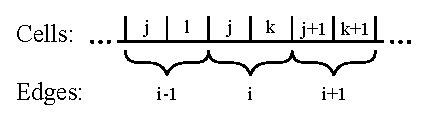
\includegraphics[width=6cm]{fig/svg/mapping.eps}
\caption{A part of the mapping from edges to cells.}
\label{fig:mapping}
\end{figure}


Some restrictions that apply is also worth noting here. The first is the use of 
only a single level of mappings. This means that every piece of data that is 
accessed during an iteration over a set is either defined directly on that set, 
or is accessed through at most one level of indirection. However, this 
restriction does not exclude applications using nested indirections, since a 
mapping table can be created to contain the indexes that we access through 
multiple mappings. The second restriction is that the result of the operations 
on the sets are independent from the order of processing the elements of the 
sets (within machine precision). This restriction enables to exploit the 
maximum opportunities for parallelization given that the accuracy of the 
algorithms do not depend on the order of execution. Finally, only  mappings with 
a fixed number of connections (or arity) are considered; such as edges to 
vertices (where the degree is always 2), unlike for a vertices to vertices 
mapping, where this will vary. The natural formalization of most FEM and FV 
algorithm uses mappings with fixed number of connections.


\subsection{Related work}\label{related-works}

Algorithms defined on unstructured meshes have been around for a long time -
discretisations such as finite volumes or finite elements often rely on these
meshes to deliver high-quality results. Indeed there is a large number of papers
detailing such algorithms, and a large number of commercial, government, and
academic research codes; to name a few OpenFOAM \cite{OpenFoamUserGuide},
Rolls-Royce Hydra \cite{moinier2002edge}, FUN3D \cite{biedron2017fun3d}. All of
these codes use unstructured meshes in some shape or form, and since they are
often used for large experiments, the efficiency of their implementation is  an
important concern. The problem of effectively parallelising applications using
unstructured meshes is far from trivial and a number of solutions can be found
in the literature.

There are a large number of papers discussing the efficient implementation and
parallelisation in classical CPU architectures
\cite{mavriplis2002parallel,jin1999openmp}, FPGAs
\cite{nagy2014accelerating,akamine2012reconfigurable}, and of course GPUs,
which is the focus of our work.

There are libraries and domain specific languages that target unstructured mesh
computations on GPUs, such as Liszt \cite{devito2011liszt}, OP2
\cite{giles2012op2}, or more specialised ones such as the OCCA\cite{libocca}
open source library by Remacle et al. \cite{remacle2016gpu}, which looks at
efficiently solving elliptic problems on unstructured hexahedral meshes. Some
of these libraries do use shared memory for improving data locality, however
advanced techniques, such as reordering and partitioning studied in this work
are not evaluated. 

In work done by Castro et al. \cite{shallow_water} on implementing
path-conservative Roe type high-order finite volume schemes to simulate shallow
flows, they also used auxiliary accumulators to avoid race conflicts while
incrementing. Wu et al. \cite{wu2013complexity} introduce caching using the
shared memory with partitioning (clustering), but they do not use colouring,
instead, they use a duplication method similar to that of Lulesh and miniAero,
as described below. Fu et al. \cite{fu2014architecting} also create contiguous
patches (blocks) in the mesh to be loaded into shared memory, although they
partition the nodes (the to-set) not the elements (the from-set of the
mapping), further, they do not load all data into shared memory, only what is
inside the patch. Writing the result back to shared memory is done by a binary
search for the column index and atomic adds, which is inefficient on the GPU. 

Mudalige et al. \cite{op2} work on the OP2 library, which is a basis of the
present work. In the CUDA implementation, they use shared memory for caching
with hierarchical colouring, but they do not reorder the threads, nor the data,
to increase data reuse.

Parallel to these works the US Department of Energy labs have released a set of
proxy applications that represent large internal production codes, showing some
of the computational and algorithmic challenges that they face. In the Lulesh
\cite{LULESH2:changes} and the miniAero \cite{miniaero} applications, two
methods are proposed to address race conflicts: the first is to allocate large
temporary arrays where the intermediate results (the increments) are placed,
avoiding any race conditions, and to use a separate kernel to gather the
results; the second is to use atomics. Both lead to increased warp divergence
and high data latencies; and the use of the temporary array also leads to much
more data being allocated and moved.

In our work, instead of porting any specific computation, we present a general
approach to accelerate unstructured mesh applications, and in particular the
indirect increment algorithmic pattern, on GPUs.
